\documentclass[t]{beamer}

% Load general definitions
% Preamble file - general definitions, package loading, etc.

%=================================
% Load packages
\usepackage{amssymb,amsmath}
\usepackage{graphicx}
\usepackage{url}
\usepackage{tikz}
\usetikzlibrary{mindmap,trees,arrows}
\usepackage{fancyvrb}
\usepackage[portuguese]{babel} 
\usepackage[utf8]{inputenc}
\usepackage{subfigure}
\usepackage{times}
\usepackage[T1]{fontenc}
\usepackage{cancel}
\usepackage{color}
\usepackage{listings}
\usepackage[document]{ragged2e}
\usepackage{hyperref}
\usepackage{listings}


%=================================
% Set mode
\mode<presentation>
{
	\usetheme{Madrid}
	\usecolortheme{structure}
	\useoutertheme{infolines}
	\setbeamercovered{invisible}
}

% Get rid of nav bar
\beamertemplatenavigationsymbolsempty

% Insert frame number at bottom of the page.
\usefoottemplate{\hfil\tiny{\color{black!90}\insertframenumber}} 

%=================================
% Define new commands

\newcommand\Real{{\mathbb{R}}}
%\newcommand{\vi}{\vspace{0.6\baselineskip}}
%\newcommand{\goodgap}{\hspace{\subfigtopskip}\hspace{\subfigbottomskip}}


% Equation environments
\newcommand{\beq}{\begin{equation}}
\newcommand{\eq}{\end{equation}}
\newcommand{\beqs}{\begin{equation*}}
\newcommand{\eqs}{\end{equation*}}
\newcommand{\beqn}{\begin{eqnarray}}
\newcommand{\eqn}{\end{eqnarray}}
% Bold variables
\newcommand{\mbf}[1]{\ensuremath{\mathbf{#1}}}
% Itemization
\newcommand{\bitem}{\begin{itemize}}
\newcommand{\eitem}{\end{itemize}}
\newcommand{\spitem}{\vskip 1em\item}
\newcommand{\bitems}{\begin{itemize}\item}
\newcommand{\benums}{\begin{enumerate}\item}
\newcommand{\eenum}{\end{enumerate}}
% color blocks
\newenvironment{colorblock}[2]{%
\setbeamercolor{block title}{#2}
\begin{block}{#1}}{\end{block}}
% Vertical spacing
\newcommand{\vone}{\vskip 1em}
\newcommand{\vhalf}{\vskip .5em}
% Frame environments
\newenvironment{ftst}[3][t]{%
\begin{frame}{environment=ftst,#1}
\frametitle{#2}
\framesubtitle{#3}}{\end{frame}}
\newenvironment{ftstf}[2]{
\begin{frame}[fragile,environment=ftstf]
\frametitle{#1}
\framesubtitle{#2}}{\end{frame}}
% colors
\definecolor{MyGray}{rgb}{0.5,0.5,0.5}
\definecolor{MyDBGray}{rgb}{0.1,0.1,0.4}
\definecolor{darkgreen}{rgb}{0,0.4,0}
\definecolor{black}{rgb}{0,0,0}
\def\defn#1{{\color{red} #1}}
% Footnote
\renewcommand{\thefootnote}{\alph{footnote}}
% Relaxed footnotes
\newcommand{\lfr}[1]{\let\thefootnote\relax\footnote{\tiny #1}}
% Verbatim environment - using FANCYVRB package
\DefineVerbatimEnvironment%
{rcode}{Verbatim}
{fontsize=\scriptsize}

% Verbatim environment - using LISTINGS package
%\lstnewenvironment{rcode} {\lstset{	language = R,
%									basicstyle = \scriptsize\ttfamily,
%									showspaces = false,
%									showstringspaces = false,
%									showtabs = false,
%									keywordstyle = \color{black}\bfseries,
%									commentstyle = \color{darkgreen},
%									numbers = none,
%									otherkeywords={	<-,
%													ggplot,
%													geom_boxplot,
%													facet_grid,
%													shapiro.test,
%													fligner.test,
%													glht,
%													with},
%									deletekeywords={data,
%													model,
%													residuals,
%													c,
%													axis,
%													default,
%													labels,
%													qq.text}}}%
%{}

% Specific definitions
\title[]{Tópicos Especiais em Computação I}
\subtitle[]{Regressão Linear}
\author[]{Patrícia Lucas\\{\footnotesize }}
\institute{Bacharelado em Sistemas de Informação \\ IFNMG  - Campus Salinas}
\date{\scriptsize Salinas\\Março 2021}

\begin{document}

\setbeamertemplate{caption}{\raggedright\insertcaption\par}
% cover page
\setbeamertemplate{footline}{}
\begin{frame}

\begin{center}
\includegraphics[width=.15\textwidth]{}
\end{center}
  \titlepage
  \begin{tikzpicture}[remember picture,overlay]
  \node[anchor=south east,xshift=-5pt,yshift=5pt] at (current page.south east) {\tiny Versão 1.2021};
  \node[anchor=south west,yshift=0pt] at (current page.south west) {
\includegraphics[width=.25\textwidth]{Logos/salinas_horizontal_jpg.jpg}};
  \end{tikzpicture}  
\end{frame}

% Main slides

\begin{ftst}{Referência}{Regressão Linear}
\begin{figure}
    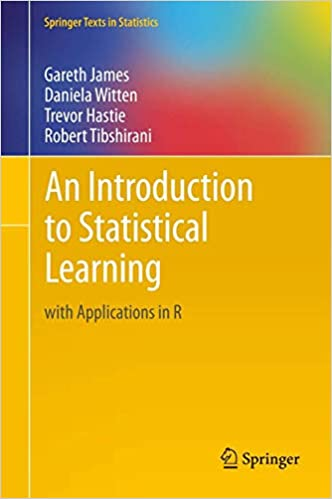
\includegraphics[scale=0.3]{Figuras/slide03_01.jpg}
\end{figure}
Capítulo 3: Linear Regression
\vone
\scriptsize

An Introduction to Statistical Learning: with Applications in R. G. James, D. Witten, T. Hastie, and R. Tibshirani. Springer, 2013.

\end{ftst}

%=====

\begin{ftst}{Regressão linear simples}{Regressão Linear}

É uma abordagem linear muito simples para prever uma resposta quantitativa $Y$ com base em uma única variável preditora $X$. 
\vone
Supõe-se que exista aproximadamente uma relação linear entre $X$ e $Y$.

\begin{equation}
    Y \approx \beta_0 + \beta_1 X
\end{equation}
\vone
$\beta_0$ e $\beta_1$ são duas constantes desconhecidas que representam os termos de interceptação e inclinação no modelo linear.
\vone
Juntos, $\beta_0$ e $\beta_1$ são conhecidos como coeficientes ou parâmetros do modelo. 

\end{ftst}

%=====

\begin{ftst}{Regressão linear simples}{Regressão Linear}

Exemplo: 
\large
\begin{equation}
    Sales \approx \beta_0 + \beta_1 TV
\end{equation}

\begin{figure}
    \centering
    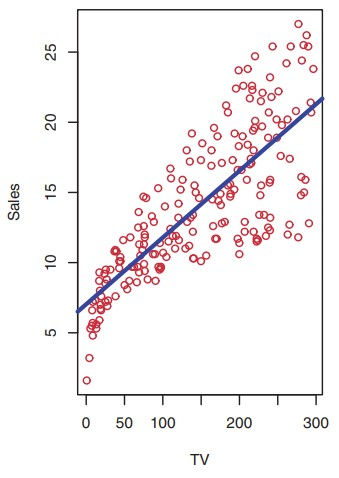
\includegraphics[scale=0.5]{Figuras/slide05_01.jpg}
\end{figure}


\end{ftst}

%=====

\begin{ftst}{Regressão linear simples}{Regressão Linear}
Na prática, $\beta_0$ e $\beta_1$ são desconhecidos. Portanto, antes de podermos usar o modelo para fazer previsões, precisamos usar dados para estimar os coeficientes.

\begin{center}
    $(x_1,y_1),(x_2,y_2), ..., (x_n,y_n)$
\end{center}
\vone
Onde $x$ são os atributos preditores (entradas) e $y$ o atributo alvo (saídas).
\vone
Nosso objetivo é obter estimativas dos coeficientes $\beta_0$ e $\beta_1$ de modo que o modelo linear se ajuste bem aos dados disponíveis.

\end{ftst}

%=====

\begin{ftst}{Regressão linear simples}{Regressão Linear}

Em outras palavras, queremos encontrar uma reta cuja interceptação $\beta_0$ e inclinação $\beta_1$, de modo que a linha resultante seja o mais próxima possível dos n pontos de dados.

\begin{figure}
    \centering
    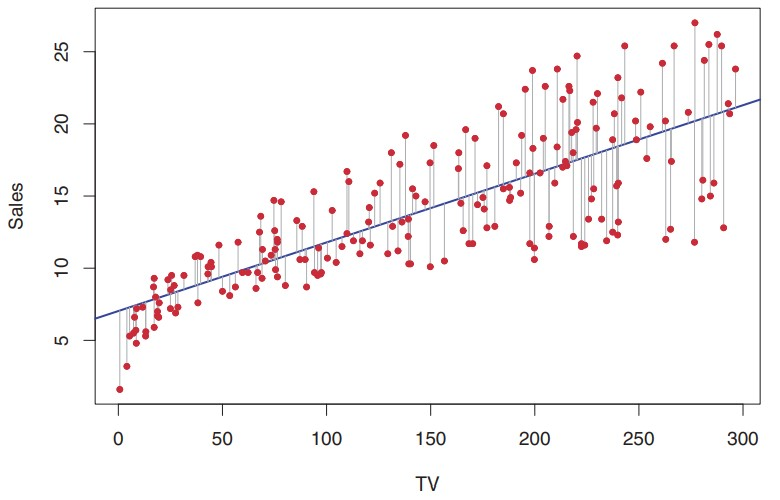
\includegraphics[scale=0.4]{Figuras/slide05_02.jpg}
\end{figure}


\end{ftst}

%=====

\begin{ftst}{Regressão linear simples}{Regressão Linear}

Existem várias maneiras de medir a proximidade, usaremos o \textbf{Método dos Mínimos Quadrados:}

\vone
Seja $\hat{y}_i = \hat{\beta}_0 + \hat{\beta}_1 x_i$ a previsão para $Y$ com base no i-ésimo valor de $X$. 
\vone
Então $\epsilon_i = y_i - \hat{y}_i$ representa o i-ésimo erro, ou seja, a diferença entre o i-ésimo valor de resposta observado e o i-ésimo valor de resposta previsto pelo modelo linear.
\vone
Definimos a soma dos erros quadráticos (SEQ) como:

\begin{equation}
    SQE = e^2_1 + e^2_2 + \ldots + e^2_n
\end{equation}
ou equivalente:
\begin{equation}
    SQE = (y_1 - \hat{\beta}_0 - \hat{\beta}_1 x_1)^2 + (y_2 - \hat{\beta}_0 - \hat{\beta}_1 x_2)^2 + \ldots + (y_n - \hat{\beta}_0 - \hat{\beta}_1 x_n)^2
\end{equation}


\end{ftst}

%=====

\begin{ftst}{Regressão linear simples}{Regressão Linear}

A abordagem dos mínimos quadrados escolhe $\hat{\beta}_0$ e $\hat{\beta}_1$ para minimizar a SEQ. Usando alguns cálculos, pode-se mostrar que os minimizadores são:
\begin{equation}
    \hat{\beta}_1 = \frac{\sum_{i=1}^n (x_i - \hat{x})(y_i - \hat{y})}
    {\sum_{i=1}^n (x_i - \hat{x})^2}
\end{equation}

\begin{equation}
    \hat{\beta}_0 = \hat{y} - \hat{\beta}_1 \hat{x}
\end{equation}

onde $\hat{y}$ e $\hat{x}$ são as médias da amostra:

\begin{equation}
    \hat{y} = \frac{1}{n} \sum_{i=1}^{n} y_i
\end{equation}

\begin{equation}
    \hat{x} = \frac{1}{n} \sum_{i=1}^{n} x_i
\end{equation}


\end{ftst}

%=====

\begin{ftst}{Regressão linear simples}{Regressão Linear}
Ajuste da regressão linear simples para os dados de Publicidade usando vendas como resposta e TV como preditor, onde $\hat{\beta}_0 = 7,03$ e $\hat{\beta}_1 = 0,0475$.
\vone
\begin{figure}
    \centering
    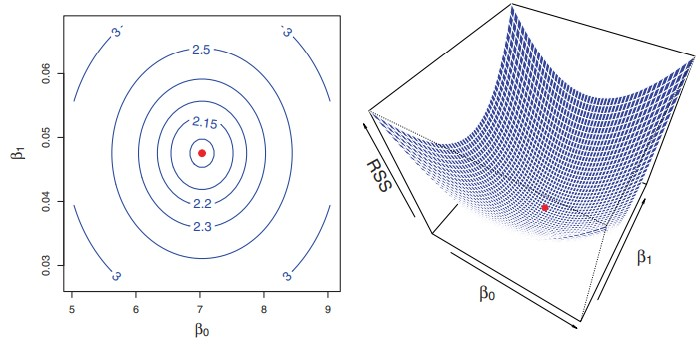
\includegraphics[scale=0.5]{Figuras/slide05_03.jpg}
\end{figure}


\end{ftst}

%=====


\end{document}